\documentclass[WHATMANUAL.tex]{subfiles}

\begin{document}

\chapter{Introduction}

\section{What is WHAT}

WHAT (Well Hydrograph Analysis Toolbox) is a free, open source, and cross-platform interactive computer program whose main focus is the interpretation of observation well hydrographs, including:

\begin{itemize}

\item the preparation of a gapless daily weather time-series (precipitation and air temperature) representative of the well location. For this purpose, an interface to the online Canadian Daily Climate Database (CDCD) is provided that allows to query stations interactively by location coordinates, download the available data, and automatically rearranged the data in a format compatible with WHAT. Furthermore, missing data for a given station can be quickly filled with data from selected neighboring weather stations using a multiple linear regression model;

\item the generation of various publication-quality figures from the weather and water level data;

\item the exploration, manipulation, and validation of the data within a user-friendly dynamic graphical environment;

\item the calculation of the master recession curve of the well hydrograph (experimental);

\item the estimation of groundwater recharge at the local scale in unconfined conditions with a method combining the daily meteorological data and the water level time series (will be available in a future release).

\item the calculation of the barometric response function of the well that can be used to assess the level of confinement of the aquifer at the well location (will be available in a future release).

\end{itemize}

WHAT is written in the Python 2.7 programming language and is currently maintained and developed by Jean-Sébastien Gosselin at INRS-ETE (\url{www.ete.inrs.ca}). The source code and a stand-alone executable for Windows 7 are available free of charge for download on GitHub (\url{https://github.com/jnsebgosselin/WHAT}). If you encounter any problems or errors during program execution, have any questions, or have specific suggestions on how to improve WHAT, please contact Jean-Sébastien Gosselin at this email address \href{mailto:jnsebgosselin@gmail.com}{jnsebgosselin@gmail.com}.

\newpage

\section{Installation}\label{sec:intallation}

WHAT can run on Windows, Linux, or OS X computer operating systems. However, a stand-alone executable of the program is currently released and tested only for the Windows 7 platform. This executable should also be compatible with Windows XP. For the Linux and OS X platforms, the software can be run directly from the source code, provided that Python 2.7 and all the required third party packages are installed on the computer (PySide, NumPy, matplotlib, xlrd, xlwt).

The stand-alone executable for Windows 7 is distributed in a Zip archive that can be downloaded freely on GitHub (\url{https://github.com/jnsebgosselin/WHAT/releases}). This archive contains:

\begin{itemize}

\item the GNU General Public License;

\item a folder named ``WHAT'' that contains all the necessary system files for the program to run, including the file ``WHAT.exe'' from which the software can be started;

\item a folder named ``Projects'' where all input and output files used or created by WHAT are stored by default. In this folder are included samples of input and output files that provide a quick and convenient way to test and learn the various features of the program.

\end{itemize}

Once the content of the Zip archive has been extracted, the program can be started directly from the WHAT.exe executable file that is contained withing the folder named WHAT. The software can conveniently run from any location on the computer or from any storage device without the need to install the program beforehand.

\section{Overview of the Graphical User Interface}
\label{sec:GUI_overview}

%There is no traditional menus in WHAT and everything is instead displayed within a menu bar that is located at the top of the interface.

WHAT Graphical User Interface (GUI) mainly consists of a menu bar, a console area, and a central view panel (see Figure~\ref{fig:WHAT_GUI}). The \emph{menu bar} is located in the top right corner of WHAT main window. This is where you can view what is the current project, open an already existing project or create a new one. The \emph{console} is located at the bottom of the WHAT interface and is used to report technical information about the various tasks accomplished by the program as well as warning and error messages. The console can be collapsed to save space, or can be extended to the entire window area. The \emph{central view panel} is the main component of the WHAT interface and is where are displayed the various features of the software. The content of this panel is divided into four tabs: \emph{Download Data}, \emph{Fill Data}, \emph{Hydrograph}, and \emph{About}. The tabs are described in a little bit more details in the text below and are shown in Figure~\ref{fig:WHAT_GUI_ScnShot}.

\begin{figure}[!ht]
\centering
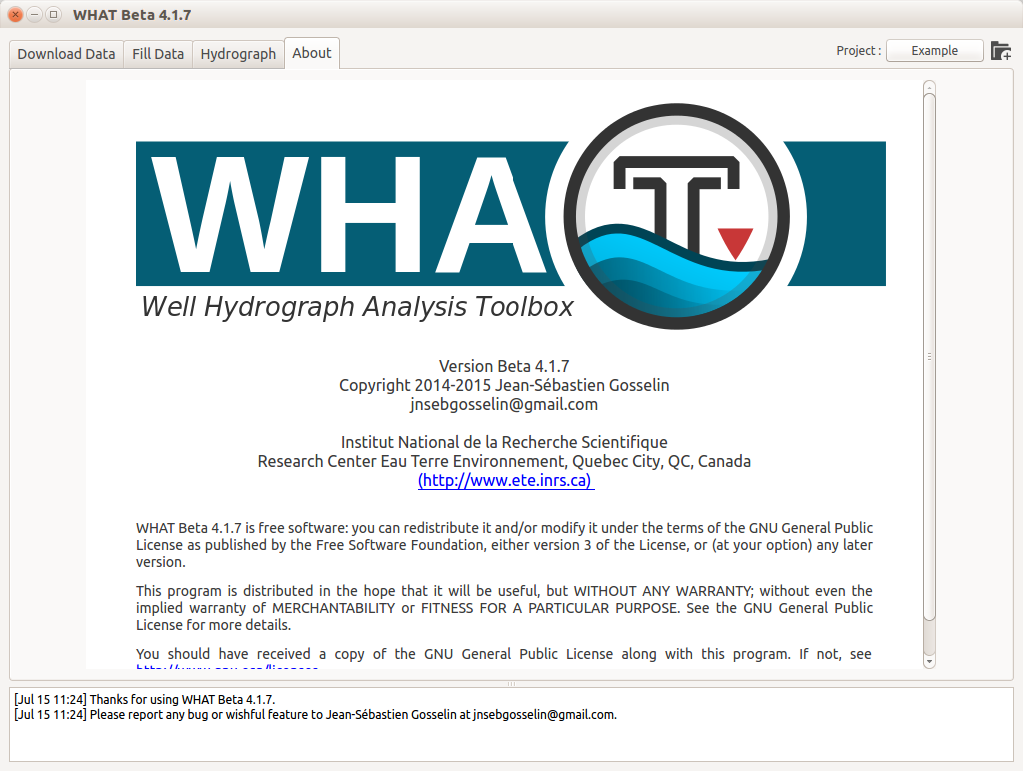
\includegraphics[width=0.75\textwidth]{img/WHAT_GUI}
\caption[WHAT GUI main features.]{WHAT GUI main features.}
\label{fig:WHAT_GUI}
\end{figure}

\newpage

\paragraph{Download Data} This tab (see Figure~\ref{subfig:ScnShot_000}) provides an interface to the online Canadian Daily Climate Database (CDCD) that allows to query stations interactively by location coordinates, download the available data, and automatically rearranged the data in a format compatible with WHAT. Alternately, it is possible to provide a custom list of Canadian weather stations for which data can be downloaded and formatted. At the moment, it is not possible to access data of weather stations located in the U.S. This feature may be added in a future release of the software.

\begin{figure}[!ht]
        \centering
        \begin{subfigure}[t]{0.45\textwidth}
                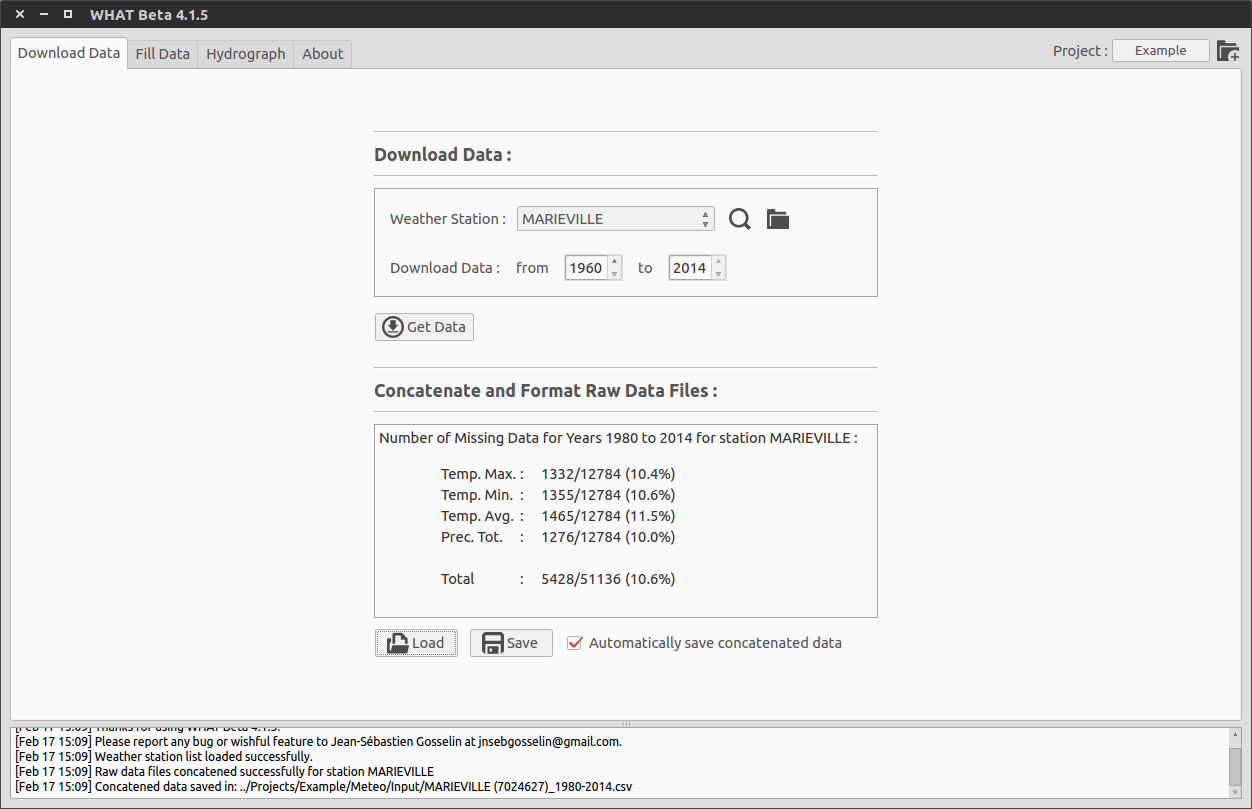
\includegraphics[width=\textwidth]{img/WHAT_Screenshot000}
                \caption{``Download Data'' tab.}
                \label{subfig:ScnShot_000}                
        \end{subfigure}%
        \hspace{0.5cm}
        \begin{subfigure}[t]{0.45\textwidth}
                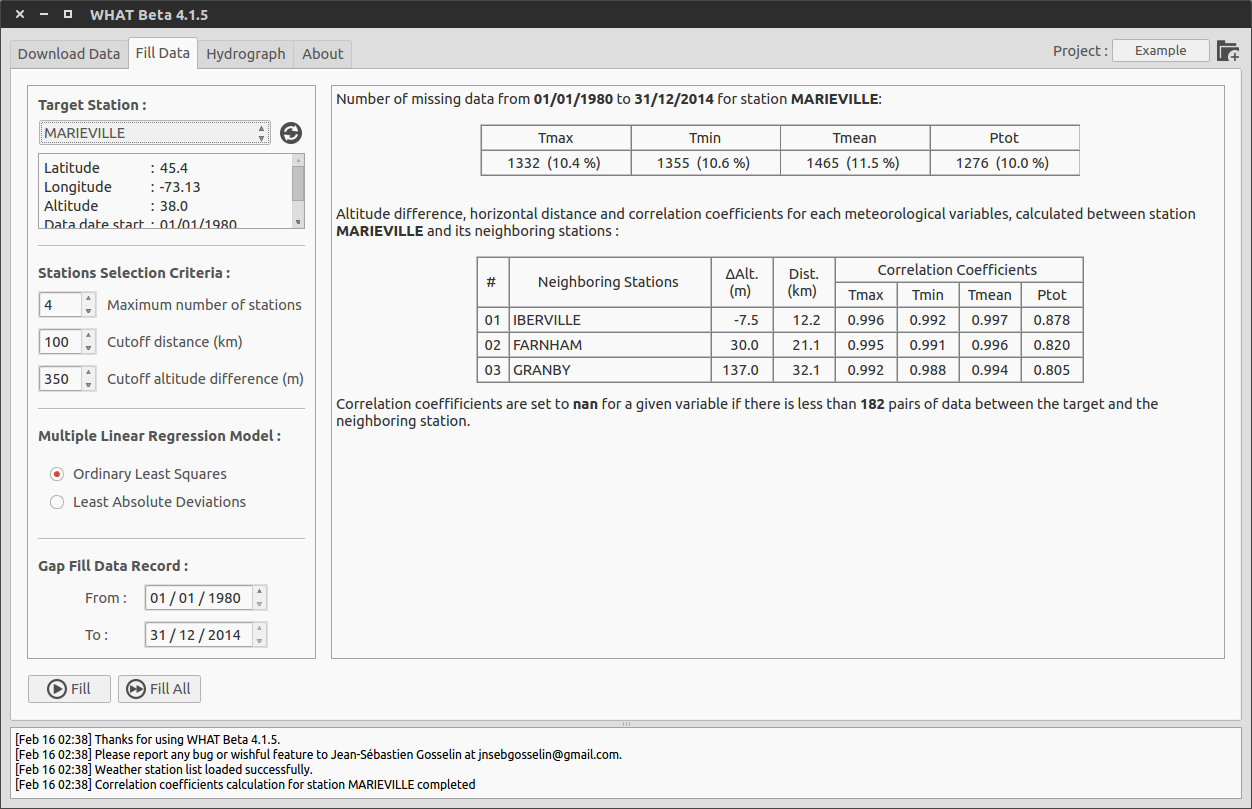
\includegraphics[width=\textwidth]{img/WHAT_Screenshot001}
                \caption{``Fill'' Data tab.}
                \label{subfig:ScnShot_001}
        \end{subfigure}
        \\[0.5cm]
        \begin{subfigure}[t]{0.45\textwidth}
                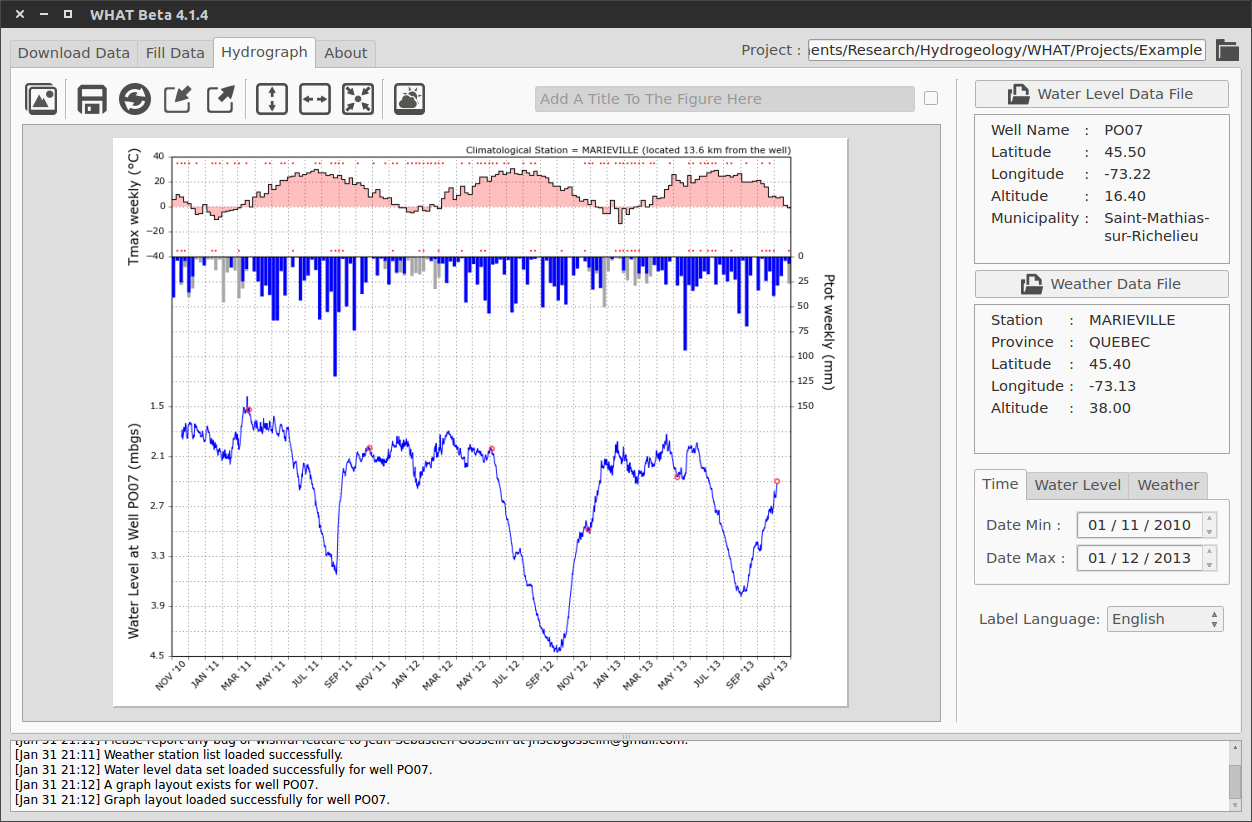
\includegraphics[width=\textwidth]{img/WHAT_Screenshot002}
                \caption{``Hydrograph'' tab in mode ``Layout''.}
                \label{subfig:ScnShot_002}
        \end{subfigure}
        \hspace{0.5cm}
        \begin{subfigure}[t]{0.45\textwidth}
                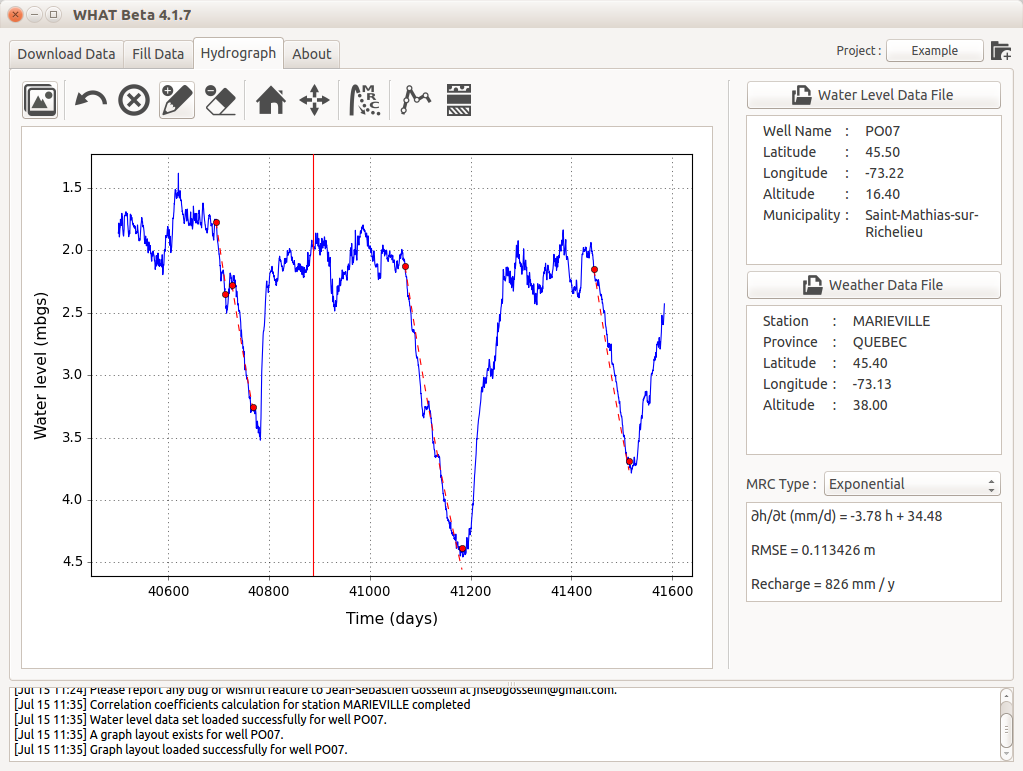
\includegraphics[width=\textwidth]{img/WHAT_Screenshot003}
                \caption{``Hydrograph'' tab in mode ``Computation''.}
                \label{subfig:ScnShot_003}
        \end{subfigure}
        \caption[Screenshots of WHAT GUI tabs captured in Ubuntu Linux 14.04.]{Screenshot of WHAT GUI tabs captured in Ubuntu Linux 14.04. (a) ``Download Data'' tab. (b) ``Fill'' Data tab (c) ``Hydrograph'' tab in mode ``Layout''. (d) ``Hydrograph'' tab in mode ``Computation''.}\label{fig:WHAT_GUI_ScnShot}
\end{figure}

\paragraph{Fill} This tab (see Figure~\ref{subfig:ScnShot_001}) is where you can automatically estimate the missing daily weather values in your data to create gapless time-series of daily precipitation and air temperature. Missing data for a given station are estimated from selected neighboring weather stations using a multiple linear regression model.

\paragraph{Hydrograph} This tab is used for viewing and plotting data. For this purpose, two modes are available: the \emph{layout} and the \emph{computation} mode. Both modes share the same weather and water level dataset and it is possible to switch from one mode to the other at anytime. The \textbf{layout} mode (see Figure~\ref{subfig:ScnShot_002}) provides an interface to interactively produce publication-quality graphs from the data. The \textbf{computation} mode (see Figure~\ref{subfig:ScnShot_003}) consists in a dynamic graphical environment where data can be explored, manipulated and analyzed. Various computational tools are available in this mode, including the estimation of the hydrograph Master Recession Curve (MRC) and the estimation of groundwater recharge.

\paragraph{About} This tab (see Figure~\ref{fig:WHAT_GUI}) displays copyright, licensing and general information about WHAT.

\section{Workflow for Interpreting Water-level Time-series}\label{sec:workflow}

WHAT is a computer software that brings together a set of tools to assist the interpretation of water level time series, from the processing of raw data to the assessment of groundwater recharge. Some are well known and documented techniques such as the estimation of missing daily weather values with the use of a multiple regression model. Others are genuine improvements of not well known or used method, such as the estimation of groundwater recharge using an approach based on the fitting of a synthetic hydrograph to real groundwater level measurements. Furthermore, WHAT has been design from the start to be modular, meaning that it will be very easy to add more tools in the future to expand the possibilities of this software.

The strength of WHAT lies not only in its various tools, but in the integration of these into a complete functional workflow for the interpretation of water level time series. This workflow is presented in Figure~\ref{fig:WHAT_workflow}. By providing a unique centralized environment where data can be processed, explored and analyzed, a lot of data manipulation and time can be saved. Moreover, the interpretation of the data is facilitated greatly, thanks to the dynamical graphical environment that is provided within the software. This is a significant improvement over the use of fragmented tools and methods, some of which are often no more than a generic spreadsheet that are not well suited for the dynamical exploration of time series.

\begin{figure}
\centering
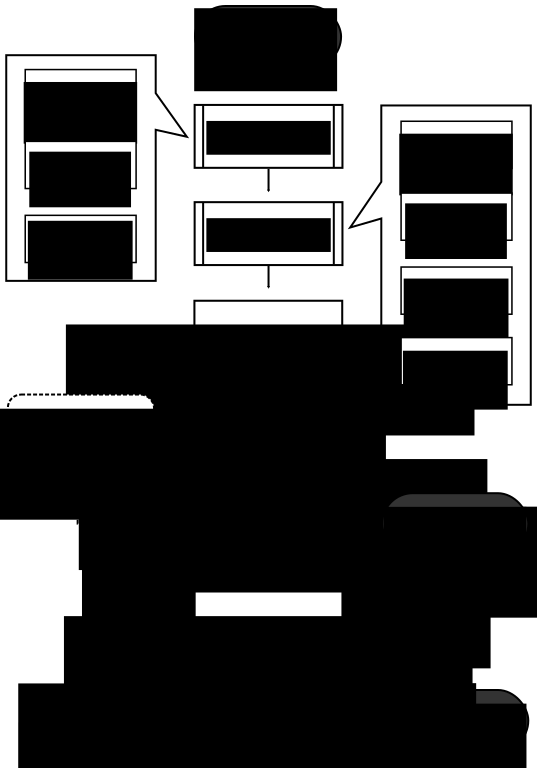
\includegraphics[height=0.95\textheight]{img/WHAT_Workflow}
\caption[WHAT workflow.]{WHAT workflow for the interpretation of groundwater-level time-series measured in an observation well or a piezometer.}
\label{fig:WHAT_workflow}
\end{figure}

The workflow shown in Figure~\ref{fig:WHAT_workflow} represents the interpretation of the data for only one well at one particular location. But, WHAT is also well suited for regional characterization projects that requires the management of data from multiple locations within a large study area. More specifically, the software allows to navigate easily through the different water level and weather datasets related to a given study area and makes the comparison of the data and the mass production of graphs and analyses efficient and easy. This can represent a substantial gain in time and data manipulation when the number of well for a given study area is important and when there is a need to update the data multiple times over the course of the project. Details about the management of projects in WHAT is presented in Section~\ref{WHAT_projects}.

The first step in the proposed workflow of Figure~\ref{fig:WHAT_workflow} for the interpretation of water level time series is the preparation of gapless weather datasets. This include downloading and formatting weather data from the CDCD database and estimating the missing daily values within each record by using data from selected neighboring stations. This step is covered in details in Section~\ref{chap:gapfilling}. The second step is the processing of the water level time series, including the validation and correction of the data. This is covered in details in Section~\ref{chap:wlvl_formatting}.

Once the weather and water level time series have been prepared, the next step consists in the production of the well hydrographs. This step is covered in details in Section~\ref{chap:plotting_data}. The plotting of the water level and weather data time-series is an important step in the interpretation process that should not be looked down since it can provide meaningful insights about the confinement conditions of the aquifer at the local and regional scale. For example, Appendix~\ref{app:confinement_cond_in_MontEst} presents an application where well hydrographs produced with an early version of WHAT were used to qualitatively deduced the confinement conditions of the regional bedrock aquifer in Monteregie Est($\sim$9000~km\textsuperscript{2}) located in southern Quebec, Canada \citep{carrier_portrait_2013}. The results from this qualitative analysis showed good agreement with the map of confinement conditions of the regional bedrock aquifer which was based on the sequence and thickness of the surficial deposits. 

Following the production of the well hydrographs, if the water level and barometric measurements were acquired at a sufficient sampling rate, it is then possible to calculate the barometric response function of the well \citep{butler_jr._new_2011,rasmussen_identifying_1997,spane_considering_2002}. This tool is very useful to characterized the confinement conditions of the aquifer around the well and also gives meaningful insights about the transmissivity of the well. This approach is discussed in Section~\ref{chap:BRF} and an example of an application to the Monteregie Est area is presented in Appendix~C base on a poster presentation by Gosselin et al.

Using the drill log of the well, the hydrograph, and the barometric response function, it should be possible to determine with a good degree of confidence if the well is in confined or unconfined conditions. For the latter case, the water level and weather data time series can be used jointly to asses the groundwater recharge of the aquifer. The first step of this task consists in the estimation of the Master Recession Curve (MRC) of the hydrograph. In the second step, groundwater recharge is estimated as the residual of a daily soil moisture balance (DSMB) model and the resulting fluxes are substituted into a mathematical model of the aquifer groundwater balance to produce a synthetic well hydrograph. The third and final step of the method consists in the calibration of the DSMB model parameters, based on the comparison of synthetic and observed well hydrographs. An example of groundwater recharge estimation is provided in Appendix~D for a well located at Rougemont in Monteregie Est, Quebec, Canada.

\end{document}